\documentclass{article}
\usepackage{forest,ctex,amsmath,color,xcolor,colortbl,graphicx,geometry,comment,listings,hyperref,booktabs,tabularx,wrapfig,caption,calc,mhchem,fix-cm,tocloft,titlesec,setspace,fancyhdr,booktabs,float,subcaption}
\usepackage{lastpage}
\usepackage[absolute,overlay]{textpos}  % 绝对定位
\setlength{\parindent}{2em} 
% ========== 标题格式定制(titlesec宏包) ========== %
\renewcommand{\thesection}{\chinese{section}}  % 一级标题编号:第X章
\renewcommand{\thesubsection}{\arabic{section}.\arabic{subsection}} % 二级:1.1
\renewcommand{\thesubsubsection}{\arabic{section}.\arabic{subsection}.\arabic{subsubsection}} % 三级:1.1.1
% 一级标题:三号黑体,居中,上下各空12pt(≈1行)
\titleformat{\section}
  [block]                  % 标题格式:display(带上下间距)
  {\centering \zihao{3} \heiti}  % 居中,三号黑体
  {\Large \thesection}       % 编号格式(Large字号,如“第一章”)
  {12pt}                     % 编号与标题的间距
  {}                         % 标题内容(无额外格式)
\titlespacing{\section}{0pt}{30pt}{30pt}  % 上间距12pt,下间距12pt

% 二级标题:四号黑体,缩进,编号显示(如“1.1”)
\titleformat{\subsection}
  {\zihao{4} \heiti}         % 四号黑体
  {\thesubsection}           % 编号(如“1.1”)
  {1em}                      % 编号与标题的间距
  {}
\titlespacing{\subsection}{0em}{1.5ex plus .5ex}{1ex plus .2ex}  % 左缩进2em

% 三级标题:小四号黑体,缩进,编号显示(如“1.1.1”)
\titleformat{\subsubsection}
  {\zihao{-4}}        % 小四号黑体(\zihao{-4}对应小四号)
  {\thesubsubsection}        % 编号(如“1.1.1”)
  {1em}                      % 编号与标题的间距
  {}
\titlespacing{\subsubsection}{0em}{1.5ex plus .5ex}{1ex plus .2ex}  % 左缩进2em


\geometry{left=2.5cm,right=2.5cm,top=2.5cm,bottom=2.5cm}
%\setlength{\parindent}{2pt} 
\date{}
\begin{document}
\vspace{-30pt}
\begin{center}
    \Large \textbf{数学建模比赛}  % 原字体可能是\Large,改为\large缩小
\end{center}
% 标题与“摘要”之间减少空白
\vspace{-13pt}
\begin{center}
    \large \textbf{摘要}  % 原字体可能是\large,改为\normalsize缩小
\end{center}
\qquad 本文针对NIPT(无创产前检测)技术中最佳检测时点选择与胎儿异常判定的问题,通过建立数学模型,对
孕妇进行合理分组并确定最佳检测策略,以最小化潜在风险并提高检测准确性。我们综合利用了数理统计等方法,
系统地解决了题目提出的四个问题。

针对问题一,首先处理表格中的数据,把检测次数不足四次的孕妇代码剔除并把检测孕周换算成天数,方便后使之后
的线性回归计算更加可靠。之后剩下的每个人的y染色体浓度与检测孕周(天数)进行\textbf{线性回归}计算方程与
$R^2$,考察到整体y染色体浓度与检测孕周的\textbf{线性拟合程度都很高}。之后对于这些人,求出检测的时间中BMI增
长速率。将每个人的线性回归程斜率与进行相关性分析,得到了一套比较显著可靠的关系模型。最后引入\textbf{斯皮尔曼系数}进行检验

针对问题二,针对问题二,本研究基于临床已知的男胎孕妇BMI是影响胎儿Y染色体浓度达标时间的主要因素,
通过对孕妇BMI进行科学分组并确定最佳NIPT检测时点,以最小化孕妇潜在风险。首先,我们依据Y染色体浓度
达标情况将孕妇分为三组:始终达标组、中间达标组和从不达标组;接着采用\textbf{K-means聚类算法}对孕妇平均BMI
进行聚类分析,通过\textbf{肘部法则}确定最佳聚类数为5类;然后计算每个BMI区间的Y染色体浓度达标时间,以中位数
确定该组最佳检测时点;最后通过\textbf{误差传播模型}分析检测误差对结果的影响。结果表明,基于BMI分组的个性化
检测时点推荐能够有效降低临床风险,为NIPT临床实践提供了科学依据。

针对问题三

针对问题四

\textbf{关键词:线性回归,斯皮尔曼系数,K-means聚类算法,肘部法则,误差传播模型}
\newpage
\section{\textbf{问题重述}}
\subsection{\textbf{问题背景}}
NIPT(Non-invasive Prenatal Testing,无创产前检测)作为一项革命性的产前筛查技术,通过采集孕
妇外周血中的胎儿游离DNA进行测序分析,能够有效评估胎儿常见染色体非整倍体异常的风险[1]。该技术具
有无创、安全、准确性高等特点,已成为临床产前筛查的重要手段。

在实际临床应用中,NIPT检测的准确性受到多种因素影响,其中胎儿游离DNA浓度(特别是Y染色体浓度对
于男胎)是关键因素之一。临床实践表明,胎儿Y染色体浓度与孕妇孕周数及身体质量指数(BMI)存在显著
相关性[2]。同时,检测时机的选择对于尽早发现胎儿异常、降低临床风险至关重要:早期发现(12周以内
)风险较低,中期发现(13-27周)风险较高,而晚期发现(28周以后)风险极高。

目前临床通常根据孕妇BMI值进行简单分组并确定统一的检测时点,但这种方法未能充分考虑孕妇年龄、体
重等个体差异,可能导致部分孕妇错过最佳检测时机,增加临床风险。因此,需要建立更加科学、个性化的
NIPT时点选择模型,为不同特征的孕妇群体制定最优检测策略。

\subsection{\textbf{问题要求}}
附件提供了某地区(大多为高BMI)孕妇的NIPT检测数据,包括孕妇年龄、BMI、孕周数、胎儿染色体浓度、
Z值、GC含量、读段数等相关指标。现需要根据这些数据建立数学模型,解决以下问题:

\textbf{问题一:}基于附件中的数据,分析胎儿Y染色体浓度与孕妇孕周数、BMI等指标的相关特性,建
立合适的数学模型描述它们之间的关系,并对模型的显著性进行统计检验。

\textbf{问题二:}临床证明男胎孕妇的BMI是影响胎儿Y染色体浓度达标时间(浓度≥4\%的最早时间)的
主要因素。请对男胎孕妇的BMI进行合理分组,确定每组的BMI区间和最佳NIPT检测时点,使得孕妇的潜在
风险最小,并分析检测误差对结果的影响。

\textbf{问题三:}综合考虑体重、年龄等多种因素对男胎Y染色体浓度达标时间的影响,同时考虑检测误
差和胎儿Y染色体浓度达标比例,根据男胎孕妇的BMI进行合理分组,确定每组的最佳NIPT检测时点,使孕
妇潜在风险最小,并分析检测误差对结果的影响。

\textbf{问题四:}针对女胎异常的判定问题,以女胎孕妇的21号、18号和13号染色体非整倍体为判定结
果,综合考虑X染色体及上述染色体的Z值、GC含量、读段数及相关比例、BMI等因素,建立女胎异常的判定
模型和方法。

\section{\textbf{问题分析}}
\subsection{\textbf{问题一的分析}}
针对问题一,我们需要先对附件中的数据进行处理,为之后对每个人进行线性回归分析,剔除掉同一个人检
测次数小于等于三的孕妇代码,使拟合结果更加可靠。之后对于每一个人,以y染色体为y轴,检测孕周(天
数)为x轴进行线性回归计算,并求$R^2$确定拟合程度。之后对与每个孕妇代码求出BMI增长率,对比斜率
与BMI增长率,检测其相关性。
\subsection{\textbf{问题二的分析}}
针对问题二,问题二要求根据男胎孕妇的BMI进行合理分组并确定最佳检测时点。我们根据Y染色体浓度是否达
标(≥4\%)将孕妇分为三类,反映不同孕妇的Y染色体浓度变化规律。然后采用K-means聚类算法对孕妇平均BMI
进行客观分组,避免主观划分的随意性。通过肘部法则确定最佳聚类数为5,确保了分组的科学性和合理性。
接着对于每个BMI分组,计算组内孕妇的Y染色体浓度达标时间(对于中间达标组采用插值法预测),以中位数
作为该组的最佳检测时点,减少异常值影响。最后考虑检测过程中可能存在的测量误差和模型误差,通过误差
传播模型评估这些误差对达标时间预测的影响程度,确保推荐时点的可靠性。


\section{\textbf{模型假设}}
1.假设附件所提供的孕妇NIPT检测数据真实、准确,且数据样本足以反映胎儿染色体浓度与孕妇孕周、BMI等指标间的统计规律。

2.假设题目中给出的Y染色体浓度4\% 的临界值是可靠且普适的。

3.假设具有相似特征(如处于同一BMI区间)的孕妇群体,其胎儿Y染色体浓度的增长规律和达标时间具有相似的统计特征。

4.假设题目所提供的特征(包括但不限于X、21、18、13号染色体的Z值、GC含量、读段数比例及孕妇BMI等)包含了足以有效判别女胎染色体是否异常的信息。

\section{\textbf{符号说明}}
\begin{table}[htbp]
    \centering
    % 列格式:第一列居中+固定宽3cm,第二列居中
    \begin{tabular*}{\linewidth}{@{\extracolsep{\fill}}>{\centering\arraybackslash}p{3cm} c}
        \toprule  % 顶部粗线
        符号 & 说明 \\
        \midrule  % 表头与内容间的细线
        $k_i^{(c)}$ & 孕妇代码为$i$的个体Y染色体浓度与孕周线性回归方程斜率 \\
        $k_i^{(b)}$ & 孕妇代码为$i$的个体BMI指数与孕周线性回归方程斜率  \\
        $c_{ij}$ & 孕妇代码为$i$的个体第$j$次检测得到的Y染色体浓度\\
        $t_{ij}$ & 孕妇代码为$i$的个体第$j$次检测的检测孕周(转化为天数)\\
        $\overline{b}$ & 所有孕妇个体BMI增长率的平均数\\
        \bottomrule  % 底部粗线
    \end{tabular*}
    \label{tab:symbols}
\end{table}

\section{\textbf{问题一模型建立求解}}
\subsection{\textbf{模型建立思路}}
问题一要求分析胎儿Y染色体浓度与孕妇孕周数和BMI等指标的相关特性。为精确刻画个体增长规律并避免群
体平均带来的偏差,我们决定采用\textbf{基于个体时间序列的线性拟合方法}。核心思路是:首先对数据
进行筛选,保证每个个体的数据点足以支持回归分析;然后为每一位符合条件的孕妇单独建立Y染色体浓度
随孕周(天数)变化的线性回归模型,以拟合斜率量化其增长速率,从而探究胎儿 Y 染色体浓度与孕妇的孕周数的关系;然后为每一位孕妇建立BMI随孕周(天数)变化的线性回归模型,并将BMI增长率与 Y 染色体浓度的增长率进行相关性分析,从而探究胎儿 Y 染色体浓度与孕妇的BMI的关系;最后综合两者,得出胎儿Y染色体浓度与孕妇孕周数和BMI的相关特性。

\subsection{\textbf{数据预处理}}
附件中的数据存在个别孕妇检测次数过少的情况,这会导致线性回归结果不可靠。为确保模型稳定性,我们
设定了数据筛选条件:仅保留检测次数大于3次的孕妇数据。

对于计算出来的结果,我们剔除掉以下拟合直线:

1.$R^2$小于0.5。此时拟合效果差。

2.斜率小于0此时Y染色体。此时浓度呈现随时间下降趋势,而经过收集资料,我们发现孕妇体内胎儿Y染色
体浓度的正常趋势是:孕早期(10-12 周)从无法检出到逐步升高→孕中期(12-22 周)稳步升至峰值→孕
晚期(>22 周)进入稳定平台期(允许轻微波动,但始终可检出) 。

经过预处理,原始数据中共包含261名孕妇的记录,其中符合要求的有效孕妇样本为178名。
\subsection{\textbf{线性回归模型}}
分析胎儿 Y 染色体浓度与孕妇的孕周数和 BMI 等指标的相关特性,本研究为每位孕妇建立了双变量时间
序列回归模型。从预处理后的有效数据中,筛选出每位孕妇多次检测的记录,分别建立以下两个一元线性
回归模型:
%公式

\textbf{1. Y染色体浓度-时间关系模型:}\\
以检测时间($t_{ij}$)为自变量,对应的Y染色体浓度($c_{ij}$)为因变量,建立回归模型:
\begin{gather}
    c_{ij}=k_i^{(c)}*t_{ij}+b_i^{(c)}+\epsilon_{ij}^{(c)} \tag{1}
\end{gather}

其中:$k_i^{(c)}$ 表示第 $i$ 位孕妇的胎儿Y染色体浓度的日增长率,这是我们关注的核心参数;
$b_i^{(c)}$ 为截距项;$\epsilon_{ij}^{(c)}$ 为随机误差项。

\textbf{2. BMI-时间关系模型:}\\
以检测时间($t_{ij}$)为自变量,对应的Y染色体浓度($c_{ij}$)为因变量,建立回归模型:
\begin{gather}
    c_{ij}=k_i^{(b)}*t_{ij}+b_i^{(b)}+\epsilon_{ij}^{(b)} \tag{2}
\end{gather}

我们采用最小二乘法进行参数估计,并计算确定系数 $R^2_i$ 以评估拟合优度
\subsection{\textbf{Y染色体浓度与时间关系的个体分析}}
基于建立的所有个体回归模型,我们首先对模型的关键参数进行了统计分析,结果如下表所示:
\begin{table}[htbp]
    \centering
    \begin{tabular*}{\linewidth}{@{\extracolsep{\fill}}c c c c}
        \toprule  % 顶部粗线
        统计量 & 斜率 $k_i$(\%/天) & 截距        & 确定系数$R_i^2$ \\
        \midrule  % 表头与内容间的细线
        平均值 & 0.000800       & -0.005467 & 0.861443    \\
        标准差 & 0.00316        & 0.038959  & 0.123487    \\
        最小值 & 0.001752       & 0.088208  & 0.999747    \\
        最大值 & 0.000205       & -0.151320 & 0.505933    \\
        \bottomrule  % 底部粗线
    \end{tabular*}
    \label{tab:crops_booktabs}
\end{table}

从表中可知,个体的Y染色体浓度均随孕天增加呈现明显的上升趋势,绝大部分模型的拟合优度较高(平均
$R^2=0.824$表明线性模型能够很好地描述浓度随时间变化的规律。
\subsection{\textbf{BMI增长率与Y染色体浓度增长率的全局相关性分析}}
为探究BMI是否导致了上述增长速率的差异,我们计算了每位孕妇的BMI增长率个体Y染色体浓度增长率 $k_i$ 的相关性。

我们绘制了标准化BMI增长速率与斜率 $k_i$ 在相应编号下的散点图
与两者在不同维度下绘制的图像,如下
%两个图并排
\begin{figure}[H]
    \centering
    % 子图1:宽度占页面的45%(左右留空)
    \begin{subfigure}[b]{0.45\textwidth}  % [b]表示底部对齐
        \centering
        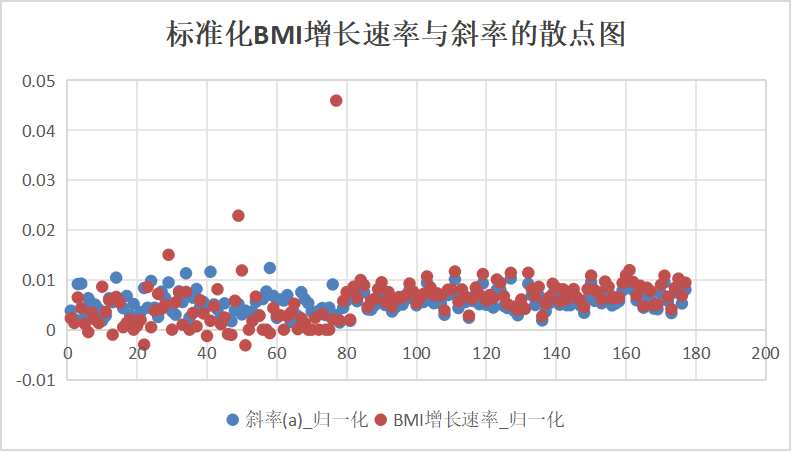
\includegraphics[width=\textwidth]{graph/biaozhunhua.png}  % 宽度=子图宽度
        \label{fig:sub1}  % 子图标签
    \end{subfigure}
    \hspace{0.05\textwidth}  % 两图间距(5%页面宽度)
    % 子图2
    \begin{subfigure}[b]{0.45\textwidth}
        \centering
        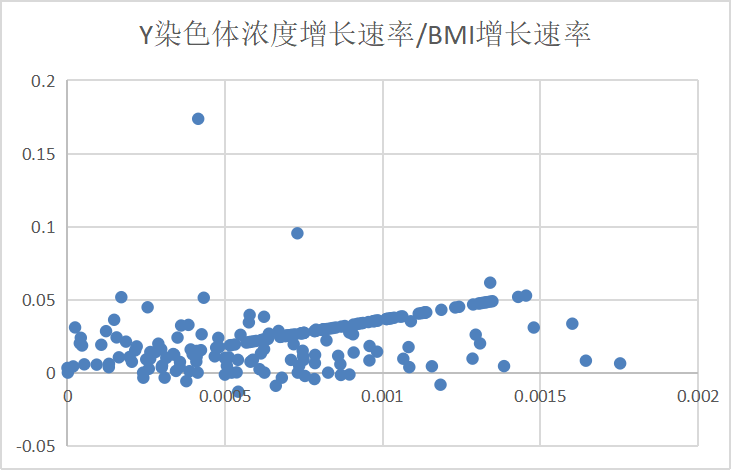
\includegraphics[width=\textwidth]{graph/erwei.png}
        \label{fig:sub2}
    \end{subfigure}
    \label{fig:two}  % 整体标签
\end{figure}
我们可以看到这两组点的吻合程度极高,由此得出结论:BMI增长率个体Y染色体浓度增长率有较高关联性。

之后,我们采用\textbf{Pearson相关系数} $r$ 来衡量二者之间的线性相关强度,并计算其显著性p值
以判断该相关性是否由随机因素引起。计算公式如下:
\textbf{Pearson相关系数计算公式:}
%公式
\begin{gather}
    r=\frac{\sum_{i=1}^{n}(b_i-\overline{b})(k_i-\overline{k})}{\sqrt{\sum_{i=1}^{n}(b_i-\overline{b})^2}\sqrt{\sum_{i=1}^{n}(k_i-\overline{k})^2}} \tag{3}
\end{gather}
其中,$n$ 为有效孕妇样本数,$b_i$ 和 $k_i$ 分别为第 $i$ 位孕妇的初始BMI和Y染色体浓度日增长率,$\overline{b}$ 和 $\bar{k}$ 分别为它们的样本均值。

\textbf{显著性检验(t检验)统计量及p值计算公式:}

为检验相关系数的显著性,构建t统计量:
\begin{gather}
    t=r\sqrt{\frac{n-2}{1-r^2}} \tag{4}
\end{gather}

我们通过上述公式计算得到r值为0.2795,p值为0.000165,满足$p < 0.001$。因此,基于统计结果,我们
有极大把握认为两者具有显著相关性。这表明,\textbf{BMI更高的孕妇,其胎儿Y染色体浓度随孕周增长的
    速度更快。}这一结论与临床经验相符,为临床上进行个性化NIPT时点预测提供了重要的数学依据。
%%%%%%%%%%%%%%%%%%%%%%%%%%%%%%%%%%%%%%%%%%%%%%%%%%%%%%%%%%%%%%%%%%%%%%%%%%%%%%%%%%%%
%%%%%%%%%%%%%%%%%%%%%%%%%%%%%%%%%%%%%%%%%%%%%%%%%%%%%%%%%%%%%%%%%%%%%%%%%%%%%%%%%%%%
%                                   QUESTION TWO                                   %
%%%%%%%%%%%%%%%%%%%%%%%%%%%%%%%%%%%%%%%%%%%%%%%%%%%%%%%%%%%%%%%%%%%%%%%%%%%%%%%%%%%%
%%%%%%%%%%%%%%%%%%%%%%%%%%%%%%%%%%%%%%%%%%%%%%%%%%%%%%%%%%%%%%%%%%%%%%%%%%%%%%%%%%%%
\section{\textbf{问题二模型建立求解}}
\subsection{\textbf{数据预处理}}
本问题旨在探究孕妇BMI对胎儿Y染色体浓度最早达标时间的影响。考虑到同一孕妇的BMI随时间变化幅度较小
(个体内变异),且个体间差异远大于时间变化量,为提高分析的准确性和可靠性,我们采用每位孕妇多次BM
I测量的平均值作为其代表值进行后续统计分析。

为合理区分样本并便于计算NIPT最佳时点,我们依据Y染色体浓度达标情况对孕妇进行了科学分组:
\begin{itemize}
    \item 第一组\textbf{(始终达标组)}:从首次检测开始Y染色体浓度即达到或超过4\%的样本。该组数据保存在 `bmi\_Y\_always\_can\_test\_result.xlsx`中,包含孕妇代码、平均BMI和最早达标天数(即首次检测时间)。
    \item 第二组\textbf{(中间达标组)}:初始检测未达标但后续检测达标的样本。该组数据保存在 \\
          `bmi\_Y\_middle\_result.xlsx`中,包含孕妇代码、平均BMI和预测达标天数(通过\textbf{插值法}计算获得,详见附录代码Line XX)。
    \item 第三组\textbf{(从不达标组)}:所有检测中Y染色体浓度均未达标的样本。该组数据保存在 \\
          `bmi\_Y\_cannot\_test\_result.xlsx`中,包含孕妇代码、平均BMI和最晚达标天数(即末次检测时间)。
\end{itemize}

为确保数据质量,若某样本曾达标但后续检测又低于4\%,则视为无效样本并予以剔除。经上述处理,最终获得
有效样本总量为230例。其中,第一组186例(占比80.87\%),第二组37例(占比16.09\%),第三组7例(占
比3.04\%)。这一分组策略确保了后续分析的可靠性和代表性。

\subsection{\textbf{BMI划分与聚类分析}}
为探究BMI对Y染色体浓度达标时间的影响模式,我们采用聚类算法对孕妇平均BMI进行科学细分。首先,通过肘
部法则确定最佳聚类数量(图1)。结果显示,当聚类数超过5时,距离平方和下降速率显著降低,故选择聚类
数k=5作为最优解。
% 单个图片
\begin{figure}[H]  % [H]表示强制当前位置(可选参数:h=此处,t=顶部,b=底部,p=单独页)
    \centering  % 图片居中
    % 插入图片:width=0.8\textwidth 表示占页面宽度的80%(可调整)
    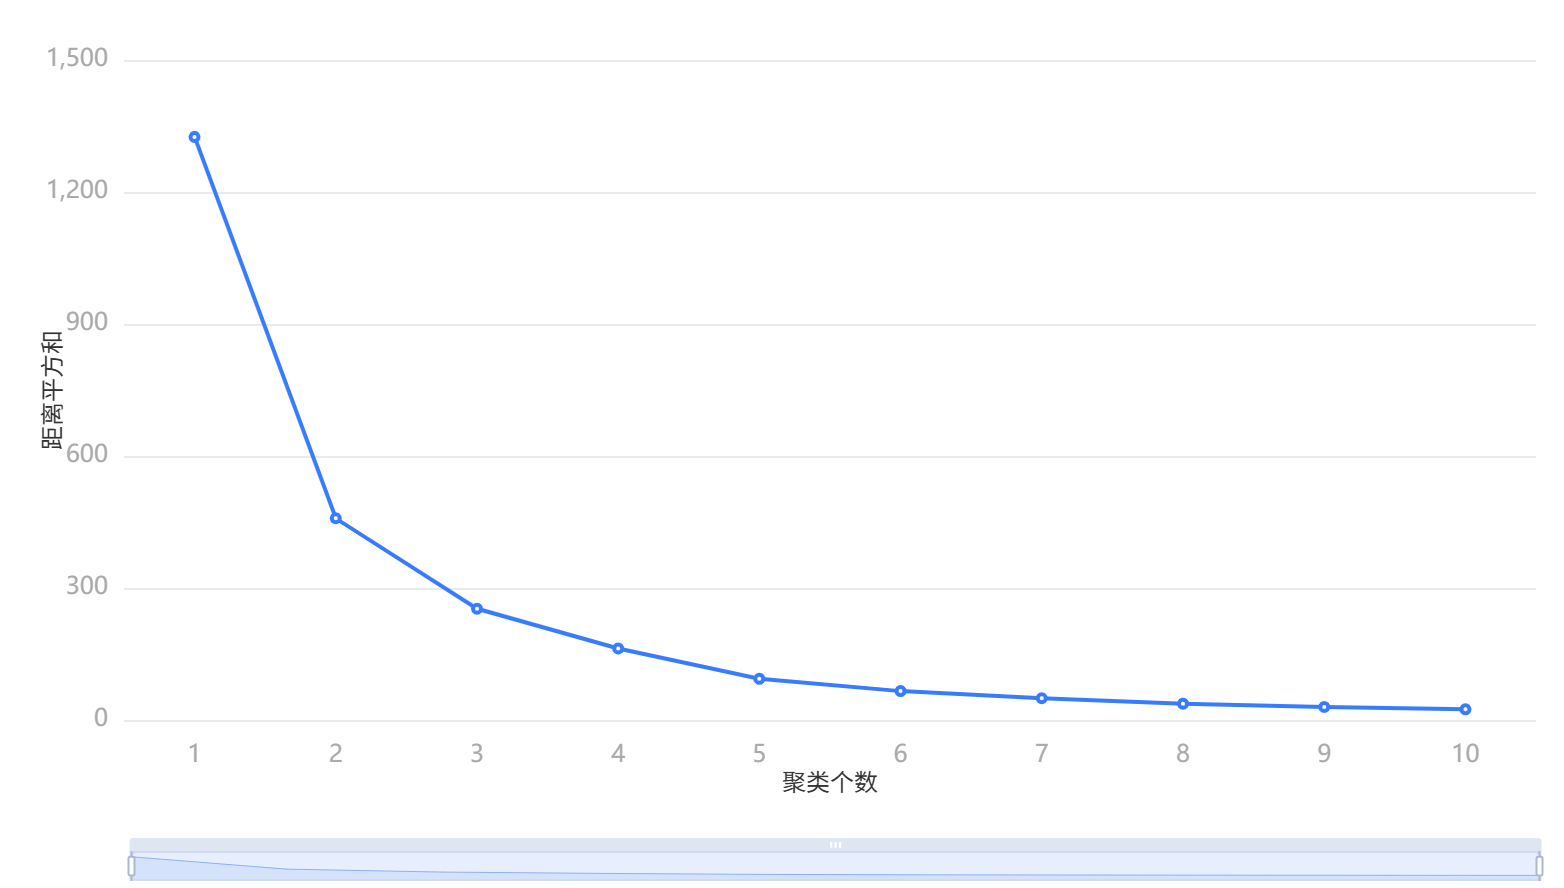
\includegraphics[width=0.8\textwidth]{graph/zhoubu.png}  % 替换为实际图片路径
    \caption{肘部法则图}  % 图片标题
    \label{fig:single}  % 标签(用于交叉引用:\ref{fig:single})
\end{figure}

基于此,我们对孕妇平均BMI与Y染色体浓度进行了K-means聚类分析,结果如图2所示。聚类结果清晰地展示
了不同BMI区间与Y染色体浓度的关联模式。
% 单个图片
\begin{figure}[H]  % [H]表示强制当前位置(可选参数:h=此处,t=顶部,b=底部,p=单独页)
    \centering  % 图片居中
    % 插入图片:width=0.8\textwidth 表示占页面宽度的80%(可调整)
    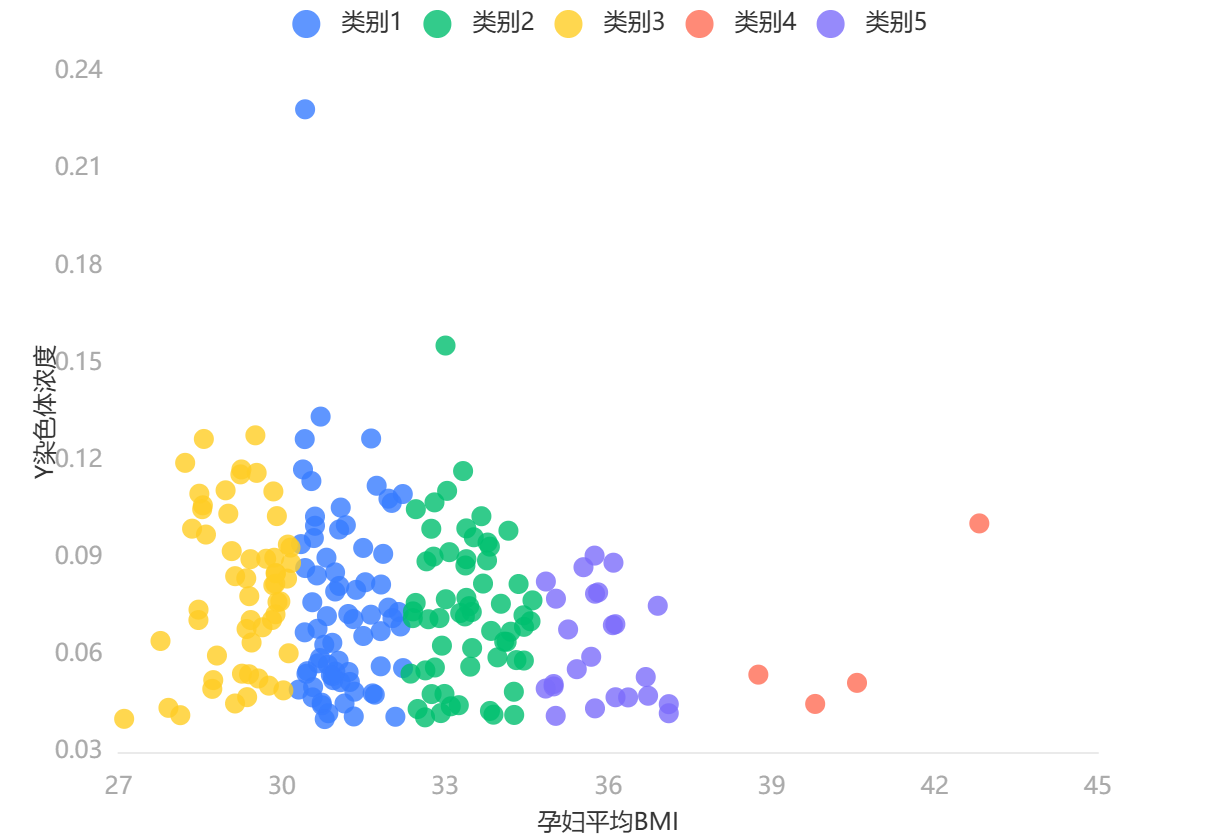
\includegraphics[width=0.8\textwidth]{graph/sandiant.png}  % 替换为实际图片路径
    \caption{聚类结果散点图}  % 图片标题
    \label{fig:single}  % 标签(用于交叉引用:\ref{fig:single})
\end{figure}

\subsection{\textbf{差异性分析与分类评价}}
为验证聚类效果,我们进行了方差分析(ANOVA)以检验不同聚类类别在各变量上的差异性,结果如表1所示。
\begin{table}[htbp]
    \centering
    \small  % 缩小字体(可选,根据需要调整)
    \setlength{\tabcolsep}{3pt}  % 减少列间距(默认约6pt)
    % 用tabularx,X型列自动分配宽度
    \begin{tabularx}{\linewidth}{X c c c c c c c}  % 第一列设为X型(自动伸缩)
        \toprule
        指标      & 类别1 $(n=71)$     & 类别2 $(n=60)$     & 类别3 $(n=55)$     & 类别4 $(n=24)$     & 类别5 $(n=4)$      & F值        & P值         \\
        \midrule
        孕妇平均BMI & $31.125\pm0.555$ & $33.415\pm0.649$ & $29.251\pm0.698$ & $35.837\pm0.716$ & $40.487\pm1.723$ & $688.969$ & $0.000***$ \\
        Y染色体浓度  & $0.076\pm0.03$   & $0.074\pm0.023$  & $0.081\pm0.024$  & $0.062\pm0.017$  & $0.063\pm0.026$  & $2.497$   & $0.044**$  \\
        \bottomrule
    \end{tabularx}
    \caption{农作物相关数据(美观版)}
    \label{tab:crops_booktabs}
\end{table}


注:***、**、*分别表示在1\%、5\%、10\%显著性水平上显著。

分析表明:
\begin{itemize}
    \item 对于变量孕妇平均BMI,显著性P值为0.000***,在1\%水平上呈现极显著差异,拒绝原假设,说明不同聚类类别间的孕妇平均BMI存在本质区别;
    \item 对于变量Y染色体浓度,显著性P值为0.044**,在5\%水平上呈现显著差异,拒绝原假设,表明不同聚类类别间的Y染色体浓度也存在统计学差异。
\end{itemize}

为进一步评估聚类质量,我们计算了三个内部评价指标:
\begin{itemize}
    \item \textbf{轮廓系数}:0.54(轮廓系数取值范围[-1,1],值越大表示同类样本越相近,不同类样本越远离,一般不可能大于0.7 )
          \begin{gather}
              s(i)=\frac{b(i)-a(i)}{\max{a(i),b(i)}} \tag{4}
          \end{gather}
          \( a(i) \): 样本 \( i \) 到\textbf{同一簇内}所有其他样本的平均距离。\textbf{(凝聚度)}
          \textbf{\( b(i) \)}: 样本 \( i \) 到\textbf{其他某个簇}的所有样本的平均距离。计算样本 \( i \)
          与所有\textbf{非本身所在簇}的的平均距离,然后取其中的\textbf{最小值}。\textbf{(分离度)}

    \item \textbf{DBI指数}:0.499(值越小表示类内紧密度越高,类间分离度越好,<0.7可接受 )
          \begin{gather}
              DBI = \frac{1}{K} \sum_{i=1}^{K} \max_{j \neq i} R_{ij} \tag{5}
          \end{gather}
          K: 簇的个数。$R_{ij}$: 簇 $i$ 和簇 $j$ 之间的\textbf{相似度}$s_i$: 簇 $i$ 的簇内散度,即簇内所有样本到其质心$c_i$的平均距离。
          $d_{ij}$: 簇 $i$ 的质心$ c_i$ 与簇$j$ 的质心 $c_j$ 之间的距离(通常使用欧氏距离)。

    \item \textbf{CH指数}:798.274(值越大表示聚类效果越优 )
          \begin{gather}
              CH = \frac{\text{SS}_B / (K - 1)}{\text{SS}_W / (N - K)}
          \end{gather}
          N: 数据集中的总样本数。K: 簇的个数。$\text{SS}_B$: \textbf{簇间离散度}(Between-Cluster Sum
          of Squares)。所有簇的质心 $c_k$ 与全局质心 $c$ 的距离平方和,并按簇大小加权。
          $\text{SS}_W$: \textbf{簇内离散度}(Within-Cluster Sum of Squares)。所有样本点到其所属簇的质心的距离平方和。

          \subsection{\textbf{NIPT时点计算}}

\end{itemize}
上述指标综合表明,本次聚类效果良好,各类别内部样本相似度高,类别之间差异明显,分类结果可靠有效,为后续分析奠定了坚实基础。
\end{document}

\begin{comment}

% 分段函数 Y_{tijk}
\[
    Y_{tijk} =
    \begin{cases}
        0, & \text{第 } i \text{ 季度未在第 } j \text{ 块地上种植物 } k \\
        1, & \text{第 } i \text{ 季度在第 } j \text{ 块地上种植物 } k
    \end{cases}
    \tag{4}
\]
\end{comment}


\begin{comment}
%公式
\begin{gather}
    X_{tijk} \leq M \cdot Y_{tijk} \quad \forall t,i,j,k \tag{5} \\
    X_{tijk} \geq 0.01 \cdot Y_{tijk} \quad \forall t,i,j,k \tag{6}
\end{gather}
\end{comment}


\begin{comment}

% 单个图片
\begin{figure}[H]  % [H]表示强制当前位置(可选参数:h=此处,t=顶部,b=底部,p=单独页)
    \centering  % 图片居中
    % 插入图片:width=0.8\textwidth 表示占页面宽度的80%(可调整)
    \includegraphics[width=0.8\textwidth]{数学建模image/屏幕截图2025-08-04185706.png}  % 替换为实际图片路径
    \caption{单张示例图片(如实验装置图)}  % 图片标题
    \label{fig:single}  % 标签(用于交叉引用:\ref{fig:single})
\end{figure}
\end{comment}


\begin{comment}
%两个图并排
\begin{figure}[H]
    \centering
    % 子图1:宽度占页面的45%(左右留空)
    \begin{subfigure}[b]{0.45\textwidth}  % [b]表示底部对齐
        \centering
        \includegraphics[width=\textwidth]{数学建模image/屏幕截图2025-08-04185706.png}  % 宽度=子图宽度
        \caption{子图1(如正面视图)}  % 子标题
        \label{fig:sub1}  % 子图标签
    \end{subfigure}
    \hspace{0.05\textwidth}  % 两图间距(5%页面宽度)
    % 子图2
    \begin{subfigure}[b]{0.45\textwidth}
        \centering
        \includegraphics[width=\textwidth]{数学建模image/屏幕截图2025-08-04185706.png}
        \caption{子图2(如侧面视图)}
        \label{fig:sub2}
    \end{subfigure}
    \caption{两张图片并排展示(整体标题)}  % 整体标题
    \label{fig:two}  % 整体标签
\end{figure}
\end{comment}


\begin{comment}
\begin{table}[htbp]
    \centering
    \begin{tabular}{ccccccccc}
        \toprule  % 顶部粗线
        作物名称                   & 地块类型    & 种植季次    & 亩产量     & 亩成本     & 销售单价    & 单位成本    & 边际收入    & 性价比     \\
        \midrule  % 表头与内容间的细线
        \cellcolor{blue!25}榆黄菇 & 普通大棚    & 第二季     & 5000    & 3000    & 57.5    & 0.60    & 95.8300 & 56.90   \\
        香菇                     & 普通大棚    & 第二季     & 4000    & 2000    & 19      & 0.50    & 38.0000 & 18.50   \\
        黄瓜                     & 普通大棚    & 第一季     & 15000   & 3500    & 7       & 0.23    & 30.0000 & 6.77    \\
        黄瓜                     & 智慧大棚    & 第二季     & 13500   & 3850    & 8.4     & 0.29    & 29.4500 & 8.11    \\
        芹菜                     & 水浇地     & 第一季     & 5500    & 900     & 4       & 0.16    & 24.4400 & 3.84    \\
        $\dots$                & $\dots$ & $\dots$ & $\dots$ & $\dots$ & $\dots$ & $\dots$ & $\dots$ & $\dots$ \\
        红薯                     & 梯田      & 单季      & 2100    & 2000    & 3.25    & 0.95    & 3.4125  & 2.30    \\
        黄豆                     & 平旱地     & 单季      & 400     & 400     & 3.25    & 1.00    & 3.2500  & 2.25    \\
        红薯                     & 山坡地     & 单季      & 2000    & 2000    & 3.25    & 1.00    & 3.2500  & 2.25    \\
        黄豆                     & 梯田      & 单季      & 380     & 400     & 3.25    & 1.05    & 3.0875  & 2.20    \\
        黄豆                     & 山坡地     & 单季      & 360     & 400     & 3.25    & 1.11    & 2.9250  & 2.14    \\
        \bottomrule  % 底部粗线
    \end{tabular}
    \caption{农作物相关数据(美观版)}
    \label{tab:crops_booktabs}
\end{table}

\end{comment}



\begin{comment}

\begin{table}[htbp]
    \centering
    \begin{tabular*}{\linewidth}{@{\extracolsep{\fill}}c c c}
        \toprule  % 顶部粗线
        作物名称    & 地块类型    & 种植季次    \\
        \midrule  % 表头与内容间的细线
        榆黄菇     & 普通大棚    & 第二季     \\
        香菇      & 普通大棚    & 第二季     \\
        黄瓜      & 普通大棚    & 第一季     \\
        黄瓜      & 智慧大棚    & 第二季     \\
        芹菜      & 水浇地     & 第一季     \\
        $\dots$ & $\dots$ & $\dots$ \\
        红薯      & 梯田      & 单季      \\
        黄豆      & 平旱地     & 单季      \\
        红薯      & 山坡地     & 单季      \\
        黄豆      & 梯田      & 单季      \\
        黄豆      & 山坡地     & 单季      \\
        \bottomrule  % 底部粗线
    \end{tabular*}
    \caption{农作物相关数据(美观版)}
    \label{tab:crops_booktabs}
\end{table}

\end{comment}
